\documentclass{article}
\usepackage{graphicx}
\usepackage[utf8]{inputenc}
\title{AuD Hausübung 5}
\date{2019-05-20}


\begin{document}
	\pagenumbering{gobble}
	\maketitle
	\newpage
	\pagenumbering{arabic}
	
	\section*{P1. (Einfügen und Löschen)}
	
	\subsection*{a)}
	\begin{figure}[h!]
		\centering
		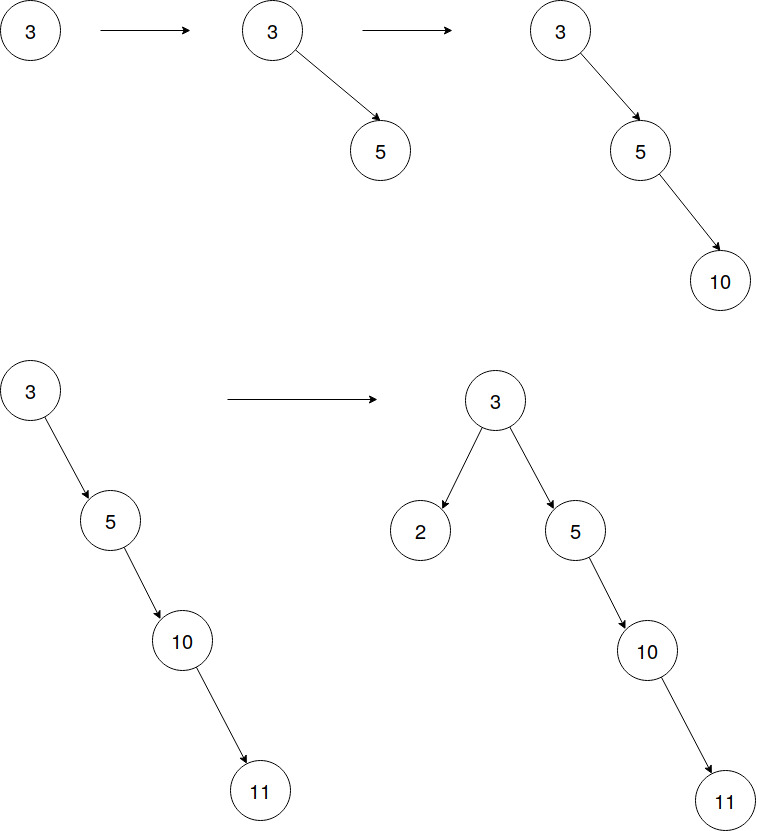
\includegraphics[width=\linewidth]{binaryTree.jpg}
	\end{figure}
	
	\newpage
	\begin{figure}[h!]
		\centering
		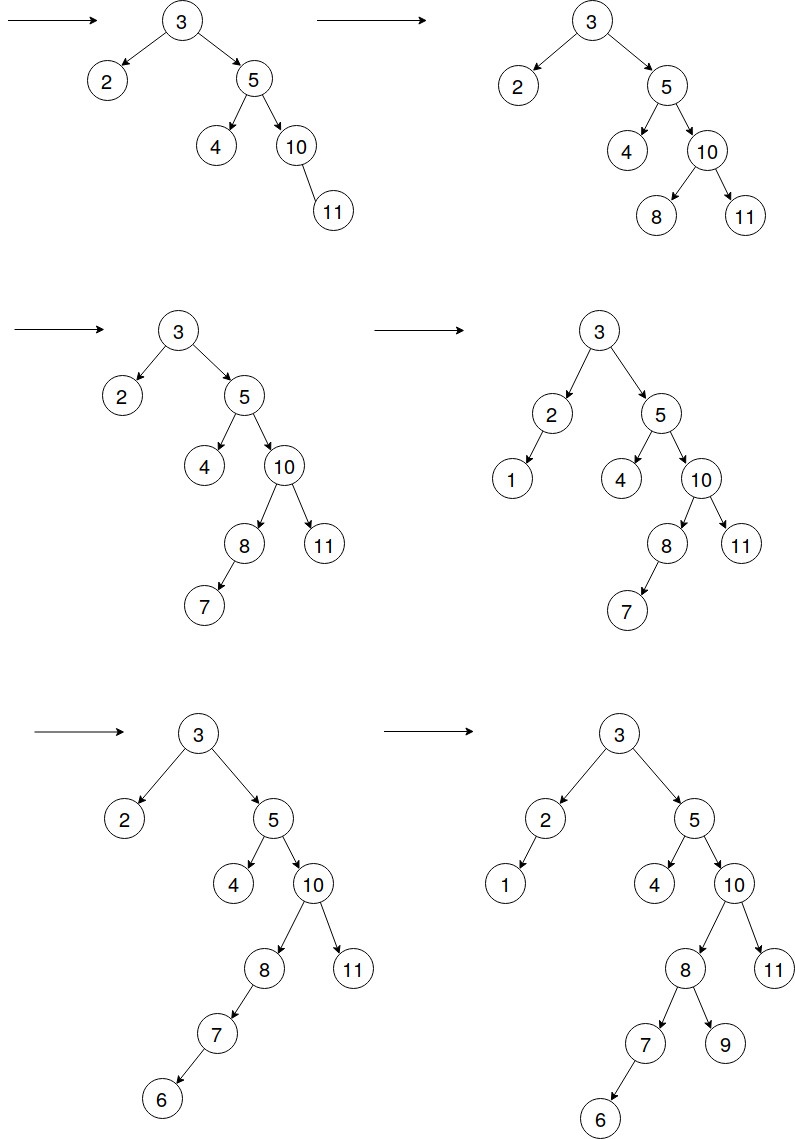
\includegraphics[width=\linewidth]{binaryTree1.jpg}
		\caption{Einfügeoperation mit den Werten 3, 5, 10, 11, 2, 4, 8, 7, 1, 6, 9}
	\end{figure}
	
	\newpage
	Der Binärbaum kann nicht als Rot-Schwarz-Baum dargestellt werden. Man betrachte den Teilbaum, der vom Knoten mit dem Wert 5 beginnt. Damit dieser Teilbaum die Schwarzhöhenregel erfüllt, müssen die Teilbäume, die von dem Kinderknoten anfangen, die gleiche Höhe haben. Das können sie aber nicht, denn der Teilbaum, der vom Knoten 4 anfängt, hat maximal eine Schwarzhöhe von 1, während der Teilbaum, der vom Knoten 10 anfängt, eine Schwarzhöhe von mindestens 2 hat. 
\end{document}
